\documentclass[12pt]{article}
\usepackage[margin=1 in]{geometry}
\usepackage{graphicx}
\usepackage{float} % For [H] figure placement
\usepackage{booktabs} % For professional tables
\usepackage{siunitx} % For SI units
\usepackage{amsmath}
\usepackage{amssymb}
\usepackage{pgfplots} % For plotting
\pgfplotsset{compat=1.18}
\usepackage{fancyhdr}
\usepackage{hyperref}
\usepackage{circuitikz} % For drawing circuits
\usepackage{subcaption}

\hypersetup{
  colorlinks=false,
  hidelinks
}
% Set paragraph formatting
\setlength{\parindent}{0in}
\setlength{\parskip}{\baselineskip}

% --- DOCUMENT INFORMATION ---
\title{Lab 10: BJT Common-Emitter Amplifier}
\author{Sean Balbale}
\date{November 30, 2025}

% --- BEGIN DOCUMENT ---
\begin{document}

% --- COVER SHEET ---
\begin{titlepage}
  \begin{center}
    \vspace*{1in}

    \Huge
    \textbf{Lab 10}

    \LARGE
    \vspace{0.5cm}
    BJT Common-Emitter Amplifier

    \vspace{3in}

    \textbf{Student Name:} Sean Balbale
    \\ \textbf{Instructor:} Debora Fixel
    \\ \textbf{Course:} ENGR 305
    \\ \textbf{Date:} November 30, 2025

    \vfill
  \end{center}
\end{titlepage}

\newpage

% --- OBJECTIVE ---
\section{Objective}
The objective of this laboratory exercise is to design, simulate, and characterize a BJT Common-Emitter (CE) amplifier. The specific goals are:
\begin{itemize}
  \item To design a CE amplifier with a specific quiescent current ($I_C = \SI{1}{mA}$) and a target voltage gain of $|A_v| = 200$ V/V.
  \item To perform a SPICE simulation to verify the DC operating point and AC small-signal performance.
  \item To build the circuit and measure the experimental gain, input/output impedances, and signal limits (clipping).
  \item To compare theoretical calculations, simulation results, and experimental measurements.
\end{itemize}

% --- THEORY ---
\section{Theory}
The Common-Emitter amplifier is a widely used configuration offering high voltage gain. In this experiment, a dual-supply topology ($V_{CC} = +15V$, $V_{EE} = -15V$) is used with an NPN transistor (2N3904).

\paragraph{DC Analysis}
The DC operating point (Q-point) determines the amplifier's region of operation. For linear amplification, the BJT must be in the active mode ($V_{BE} \approx 0.7V$ and $V_{CE} > 0.2V$).
The DC emitter current is determined by the emitter resistor $R_E$:
$$
I_E \approx \frac{V_B - V_{BE} - V_{EE}}{R_E}
$$
Assuming the base is at DC ground ($V_B \approx 0V$) and $V_{BE} \approx 0.7V$, $R_E$ sets the bias current. The collector current is $I_C \approx I_E$.

\paragraph{AC Small-Signal Analysis}
The voltage gain $A_v$ of a bypassed CE amplifier (where the emitter resistor is bypassed by a capacitor $C_E$ to ground) is given by:
$$
A_v = -g_m (R_C \parallel R_L)
$$
where $g_m$ is the transconductance of the BJT:
$$
g_m = \frac{I_C}{V_T} \approx \frac{I_C}{\SI{26}{mV}}
$$
The negative sign indicates a $180^{\circ}$ phase shift.
The output resistance $R_o$ of the amplifier (looking into the collector) is dominated by the collector resistor $R_C$, assuming the transistor's Early resistance $r_o$ is large ($r_o \gg R_C$).
$$
R_o \approx R_C
$$

% --- EXPERIMENTAL METHOD ---
\section{Experimental Method and Design}

\subsection{Design Procedure}
The circuit was designed to meet the following specifications:
\begin{itemize}
  \item $V_{CC} = +15V$, $V_{EE} = -15V$.
  \item Load Resistance $R_L = \SI{10}{k\Omega}$.
  \item Quiescent Current $I_C = \SI{1}{mA}$.
  \item Magnitude of Voltage Gain $|A_v| = 200$.
\end{itemize}

\textbf{1. Calculating $R_E$:}
To achieve $I_C \approx I_E = \SI{1}{mA}$ with the base at ground:
$$ R_E = \frac{0V - 0.7V - (-15V)}{\SI{1}{mA}} = \frac{14.3V}{\SI{1}{mA}} = \SI{14.3}{k\Omega} $$
(Standard value chosen: $14.3 \text{ k}\Omega$).

\textbf{2. Calculating $R_C$:}
The transconductance is $g_m = \frac{1\text{ mA}}{26\text{ mV}} = \SI{38.46}{mS}$.
Using the gain equation $|A_v| = g_m (R_C \parallel R_L)$:
$$ 200 = (38.46 \times 10^{-3}) \left( \frac{R_C \cdot 10k}{R_C + 10k} \right) $$
Solving for the equivalent AC load: $R_{AC} = \frac{200}{0.03846} = \SI{5.2}{k\Omega}$.
$$ \frac{1}{R_C} = \frac{1}{5.2k} - \frac{1}{10k} \implies R_C \approx \SI{10.83}{k\Omega} $$
(Standard value chosen: $10.8 \text{ k}\Omega$).

\subsection{Schematic}
The complete schematic used for simulation and prototyping is shown below.

\begin{figure}[H]
  \centering
  \begin{circuitikz}[american, scale=0.9, transform shape]
    % --- Coordinates ---
    % Define the main transistor position
    \node[npn](Q1) at (6, 0) {2N3904};

    % --- Power Rails (Vertical Alignment) ---
    \draw (Q1.C) -- ++(0, 0.5) coordinate(CNode);
    \draw (CNode) to[R, l=$R_C$, a=$\SI{10.83}{k\ohm}$] ++(0, 3) node[vcc]{$V_+ = \SI{15}{V}$};

    \draw (Q1.E) -- ++(0, -0.5) coordinate(ENode);
    \draw (ENode) to[R, l=$R_E$, a=$\SI{14.06}{k\ohm}$] ++(0, -3) node[vee]{$V_- = \SI{-15}{V}$};

    % --- Input Stage (Left Side) ---
    % Horizontal path: Source -> Rsig -> Cc1 -> Base
    \draw (Q1.B) -- ++(-1, 0) coordinate(BaseNode); % Node for RB connection

    % RB to Ground (Vertical drop)
    \draw (BaseNode) to[R, l=$R_B$, a=$\SI{10}{k\ohm}$] (BaseNode |- 0, -4) node[ground]{};

    % Input path continuing left
    \draw (BaseNode) to[C, l=$C_{c1}$, a=$\SI{47}{\micro\farad}$] ++(-3, 0) coordinate(C1Node);
    \draw (C1Node) to[R, l=$R_{sig}$, a=$\SI{50}{\ohm}$] ++(-3, 0) coordinate(InNode);

    % Source to Ground
    \draw (InNode) to[sV, l=$v_{sig}$] (InNode |- 0, -4) node[ground]{};

    % --- Output Stage (Right Side) ---
    % Horizontal path: Collector -> Cc2 -> Output
    \draw (CNode) to[short, *-] ++(0,0) -- ++(1.5, 0) coordinate(C2Start);
    \draw (C2Start) to[C, l=$C_{c2}$, a=$\SI{47}{\micro\farad}$] ++(2.5, 0) coordinate(OutNode);

    % Output label
    \draw (OutNode) to[short, -o] ++(0.5, 0) node[right]{$v_o$};

    % RL to Ground (Vertical drop from Output Node)
    \draw (OutNode) to[R, l=$R_L$, a=$\SI{10}{k\ohm}$] (OutNode |- 0, -4) node[ground]{};

    % --- Emitter Bypass (Right Side) ---
    % Connection from Emitter Node -> Right -> Down through CE -> Ground
    % This matches the visual style of placing shunts vertically
    \draw (ENode) to[short, *-] ++(2, 0) coordinate(ECapNode);
    \draw (ECapNode) to[C, l=$C_E$, a=$\SI{47}{\micro\farad}$] (ECapNode |- 0, -4) node[ground]{};

  \end{circuitikz}
  \caption{Schematic of the Common-Emitter Amplifier.}
  \label{fig:schematic}
\end{figure}

\subsection{Experimental Setup}
The circuit was constructed on a breadboard as shown in Figure \ref{fig:breadboard}.
The exact measured values of the components used were: $R_C = \SI{10.74}{k\Omega}$, $R_E = \SI{14.15}{k\Omega}$, $R_{sig} = \SI{46.1}{\Omega}$, and $R_L = \SI{9.87}{k\Omega}$.

\begin{figure}[H]
  \centering
  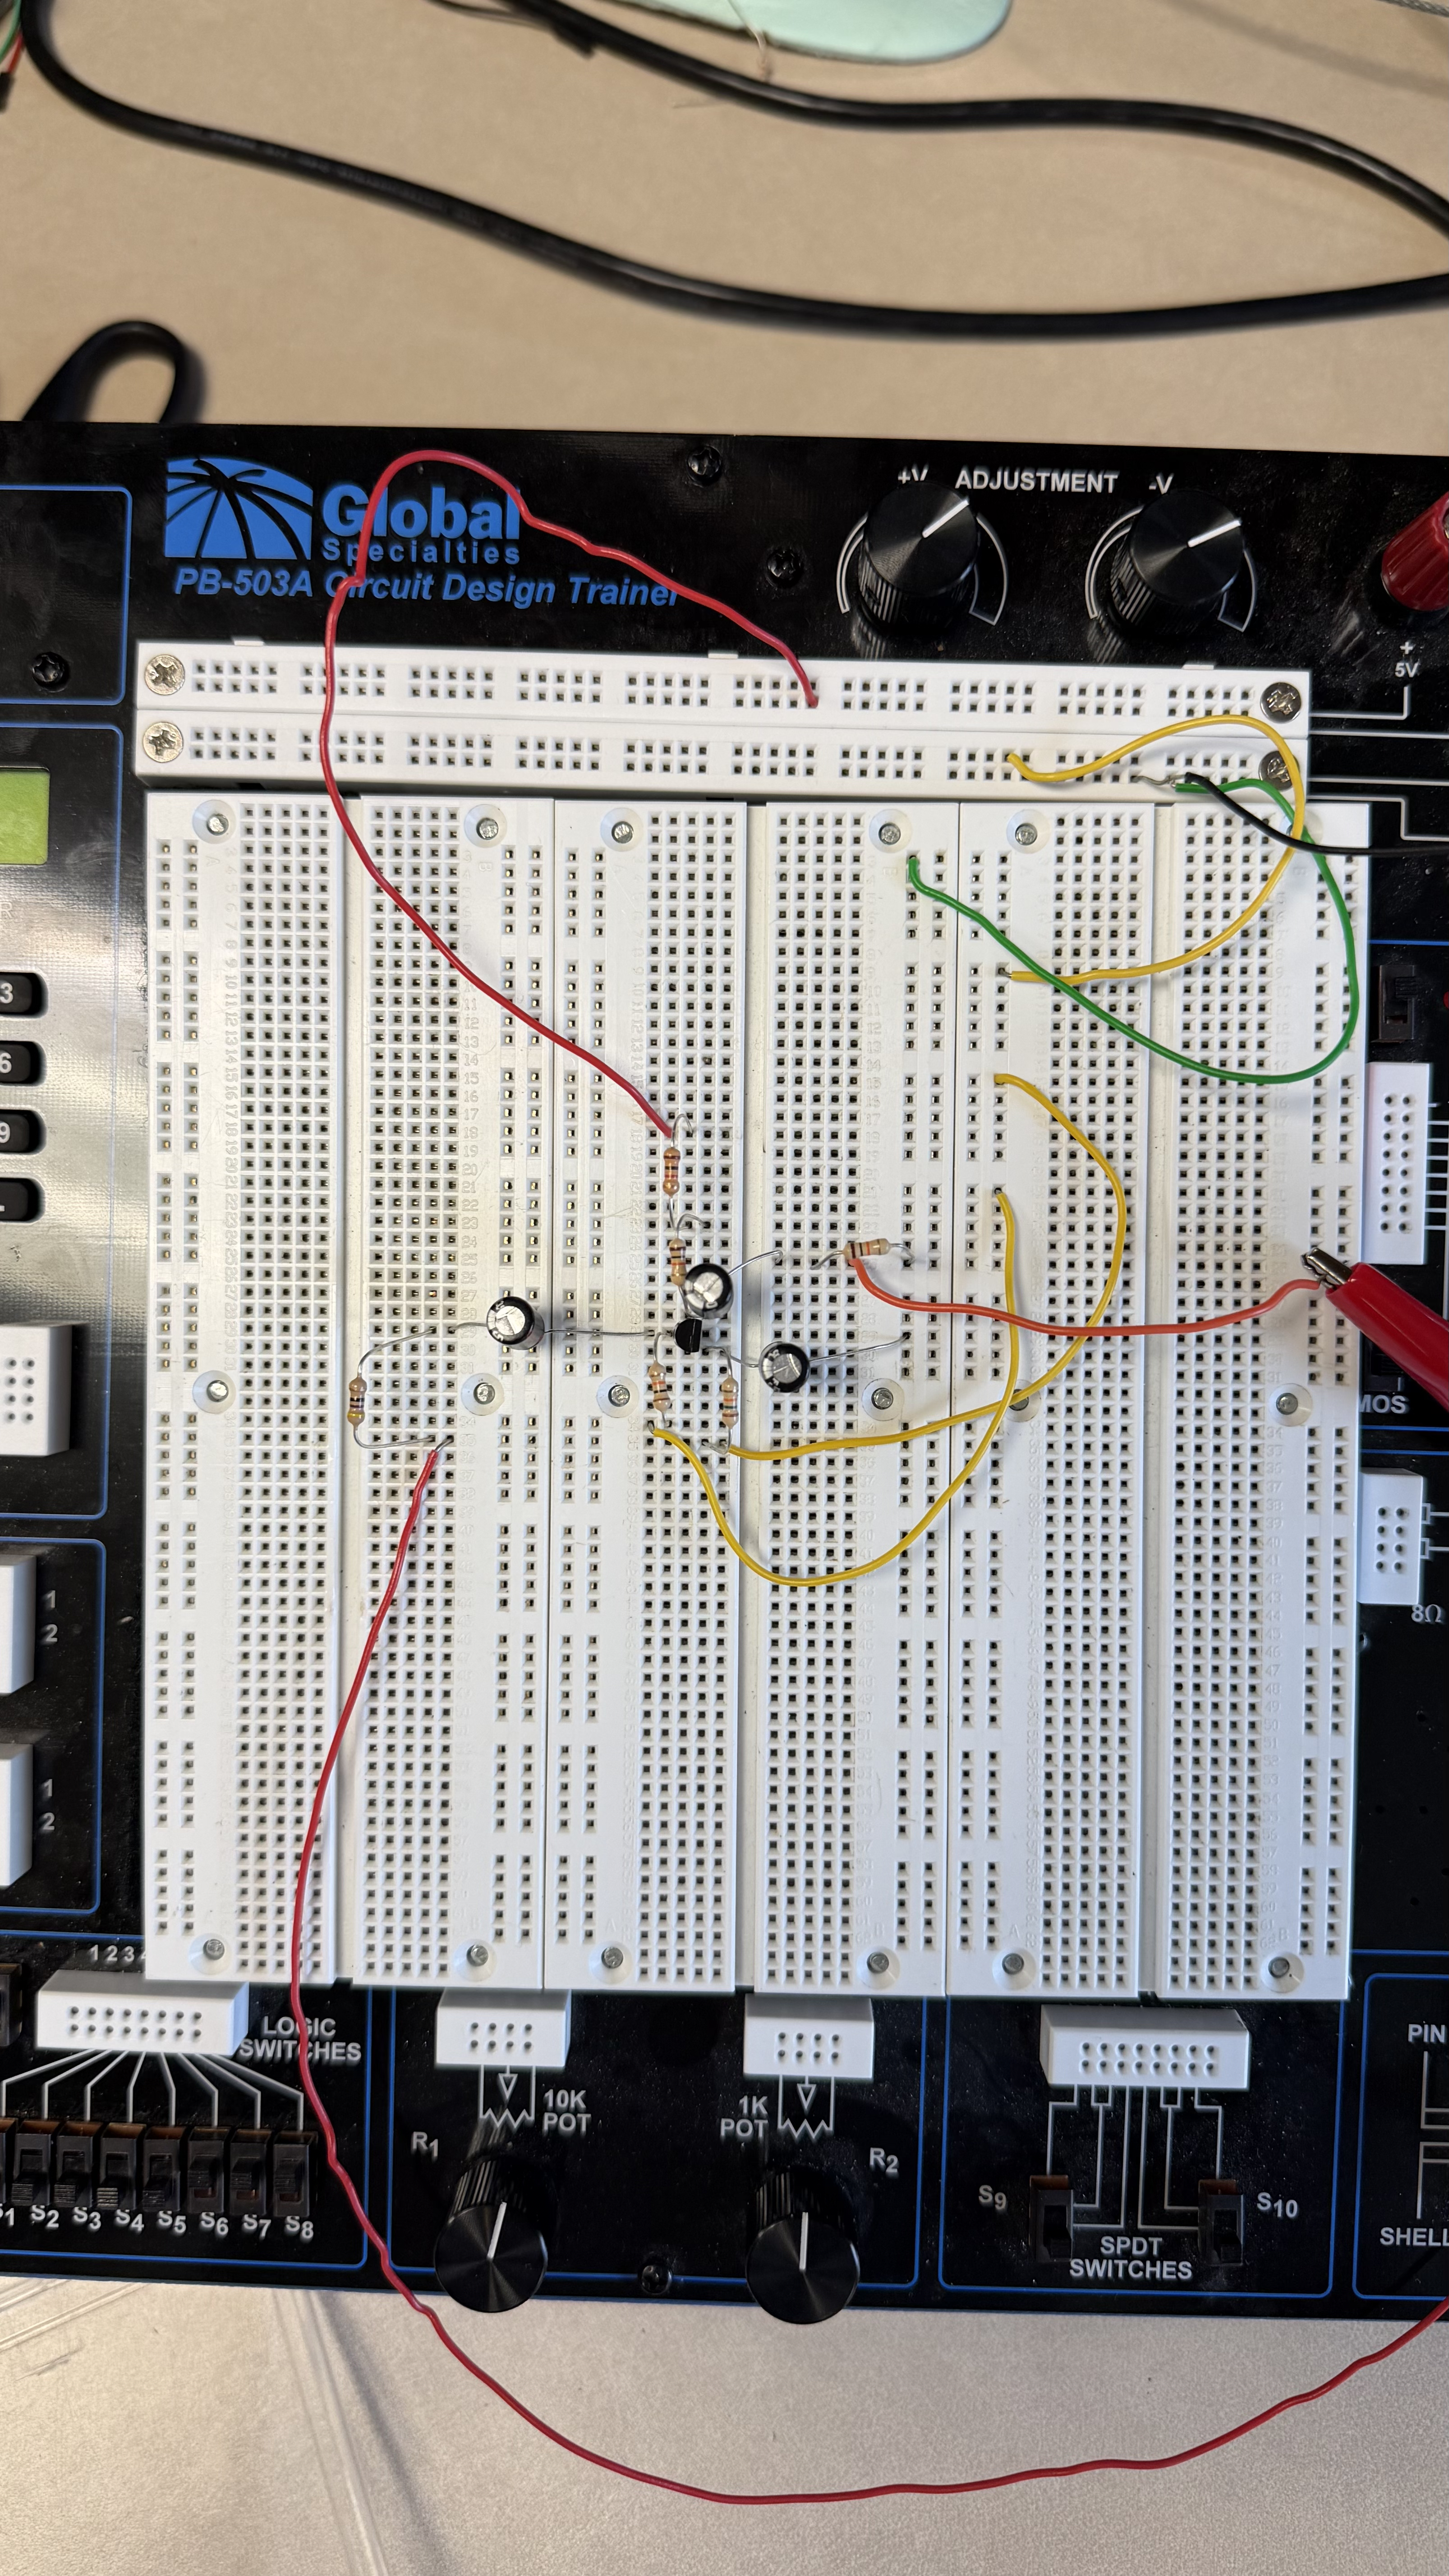
\includegraphics[width=0.6\textwidth]{IMG_0883.png}
  \caption{The assembled Common-Emitter amplifier on the breadboard.}
  \label{fig:breadboard}
\end{figure}

% --- RESULTS AND DISCUSSION ---
\section{Results and Discussion}

\subsection{DC Operating Point}
The DC voltages and currents are summarized below. As requested by the lab manual, the values for $V_{BE}$, $V_{CE}$, $I_C$, and $I_E$ are explicitly compared.

\begin{table}[H]
  \centering
  \caption{DC Operating Point Analysis: Comparison of Calculated, Simulated, and Measured Values}
  \label{tab:dc_compare}
  \sisetup{round-mode=places,round-precision=3}
  \begin{tabular}{lccc}
    \toprule
    \textbf{Parameter} & \textbf{Calculated} & \textbf{Simulated} & \textbf{Measured} \\
    \midrule
    $V_C$ & \SI{4.17}{\volt} & \SI{4.01}{\volt} & \SI{4.17}{\volt} \\
    $V_E$ & \SI{-0.7}{\volt} & \SI{-0.687}{\volt} & \SI{-0.718}{\volt} \\
    $V_B$ & \SI{0}{\volt} & \SI{-0.033}{\volt} & \SI{-0.017}{\volt} \\
    \midrule
    $\mathbf{V_{BE}}$ ($V_B - V_E$) & \SI{0.7}{\volt} & \SI{0.655}{\volt} & \SI{0.701}{\volt} \\
    $\mathbf{V_{CE}}$ ($V_C - V_E$) & \SI{4.87}{\volt} & \SI{4.70}{\volt} & \SI{4.888}{\volt} \\
    $\mathbf{I_C}$ & \SI{1.0}{\milli\ampere} & \SI{1.01}{\milli\ampere} & \SI{1.01}{\milli\ampere} \\
    $\mathbf{I_E}$ & \SI{1.0}{\milli\ampere} & \SI{1.01}{\milli\ampere} & \SI{1.01}{\milli\ampere} \\
    \bottomrule
  \end{tabular}
\end{table}

\textbf{Analysis of DC Values:}
\begin{itemize}
  \item \textbf{$V_{BE}$:} The measured Base-Emitter voltage ($\SI{0.701}{V}$) is almost exactly the standard theoretical turn-on voltage of $\SI{0.7}{V}$. The simulation predicted a slightly lower turn-on voltage ($\approx \SI{0.65}{V}$), which is typical for the SPICE model at low currents.
  \item \textbf{$V_{CE}$:} The measured Collector-Emitter voltage ($\SI{4.888}{V}$) matches the design goal ($\SI{4.87}{V}$) exceptionally well, confirming the transistor is biased correctly in the forward-active region.
  \item \textbf{Currents:} The measured currents ($I_C$ and $I_E$) are within $1\%$ of the $\SI{1}{mA}$ design target.
\end{itemize}

\subsection{AC Performance and Gain}

\begin{figure}[H]
  \centering
  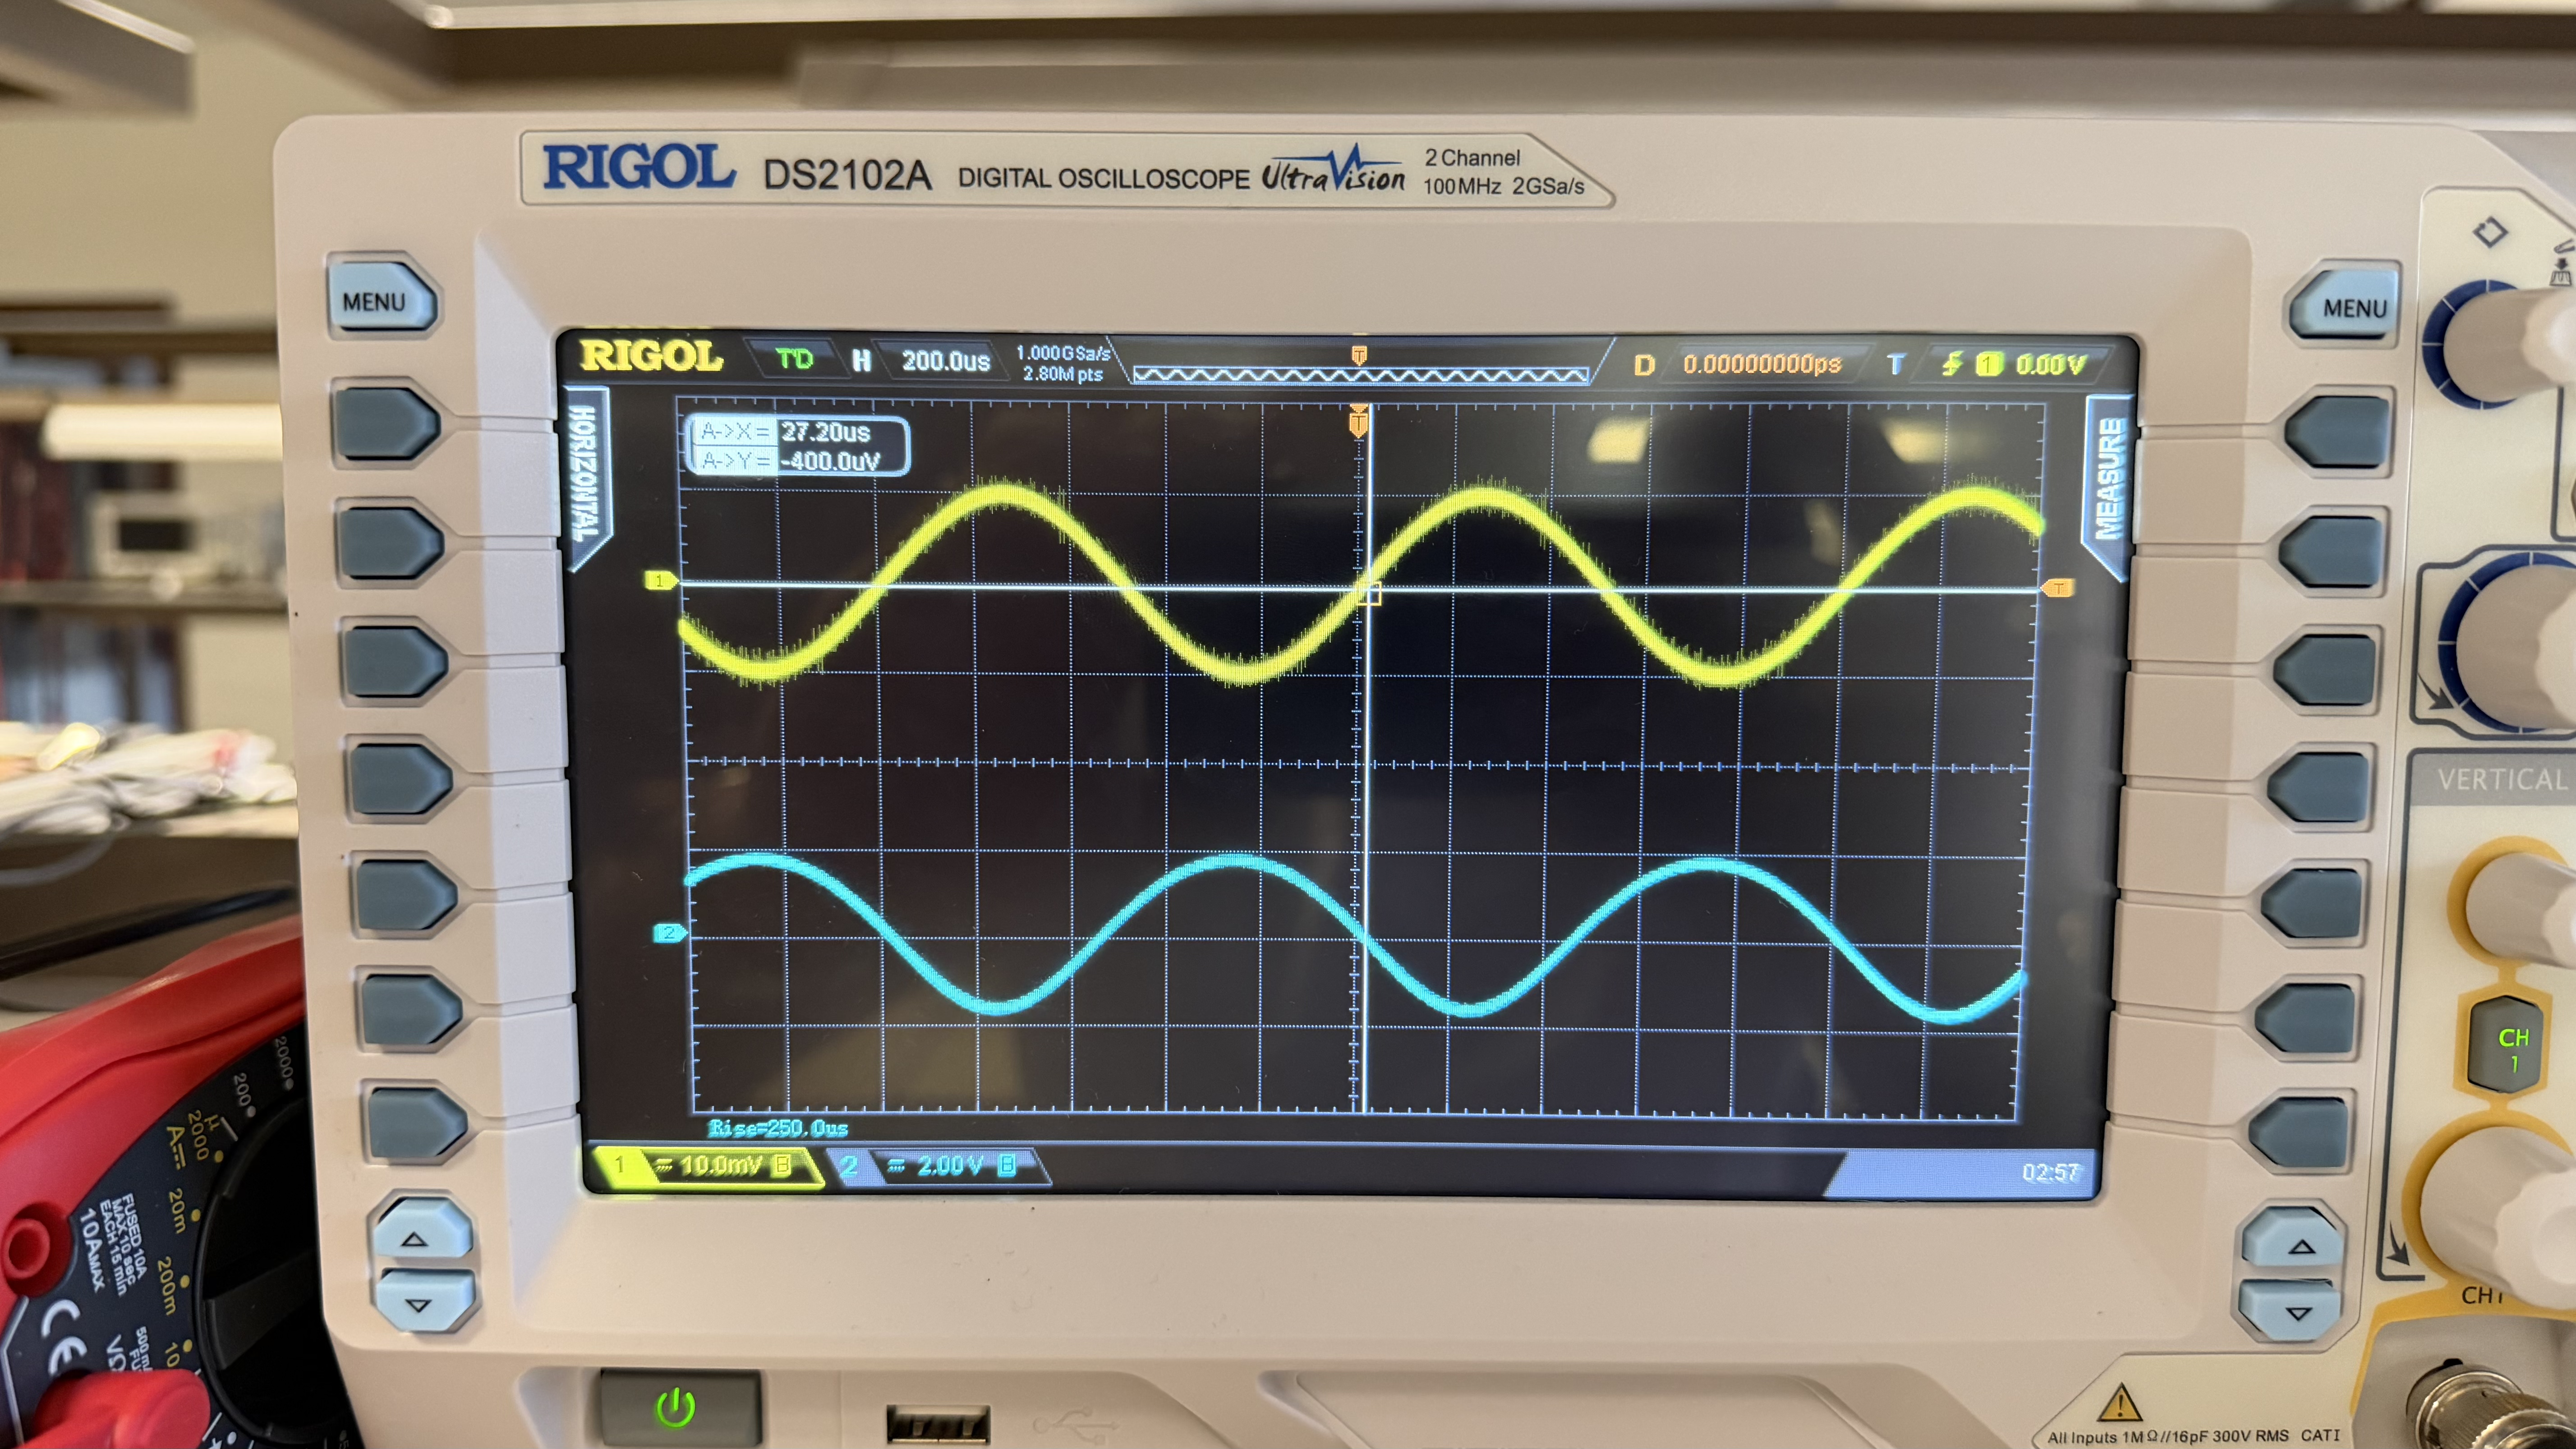
\includegraphics[width=0.7\textwidth]{IMG_0890.png}
  \caption{Oscilloscope measurement of Gain with $R_L = \SI{9.87}{k\Omega}$. Input (Yellow) and Output (Blue).}
  \label{fig:gain_meas}
\end{figure}

\begin{table}[H]
  \centering
  \caption{AC Performance Comparison}
  \label{tab:ac_compare}
  \begin{tabular}{lccc}
    \toprule
    \textbf{Parameter} & \textbf{Design Goal} & \textbf{Simulated} & \textbf{Measured} \\
    \midrule
    Input ($v_{in}$) & -- & $10 \text{ mV}_{\text{pp}}$ & $24.8 \text{ mV}_{\text{pp}}$ \\
    Output ($v_{out}$) & -- & $1.90 \text{ V}_{\text{pp}}$ & $4.88 \text{ V}_{\text{pp}}$ \\
    \textbf{Gain ($A_v$)} & \textbf{-200 V/V} & \textbf{-190 V/V} & \textbf{-196.8 V/V} \\
    \bottomrule
  \end{tabular}
\end{table}

\textbf{Gain Analysis:}
The measured gain of $\mathbf{-196.8 \text{ V/V}}$ is incredibly close to the design goal of 200 (error $< 1.6\%$).
\begin{itemize}
  \item \textbf{vs. Calculation:} The match is near perfect, suggesting the transconductance estimate ($g_m \approx I_C/V_T$) held true.
  \item \textbf{vs. Simulation:} The measured gain was slightly higher than the simulated gain (190). The simulation likely assumes a lower Early Voltage ($V_A$) for the generic 2N3904 model, which would lower the effective output impedance and thus the gain.
\end{itemize}

\subsection{Output Resistance ($R_o$)}
The output resistance was determined experimentally by comparing the "Open Load" output voltage to the "Loaded" output voltage.

\begin{figure}[H]
  \centering
  \begin{subfigure}{0.48\textwidth}
    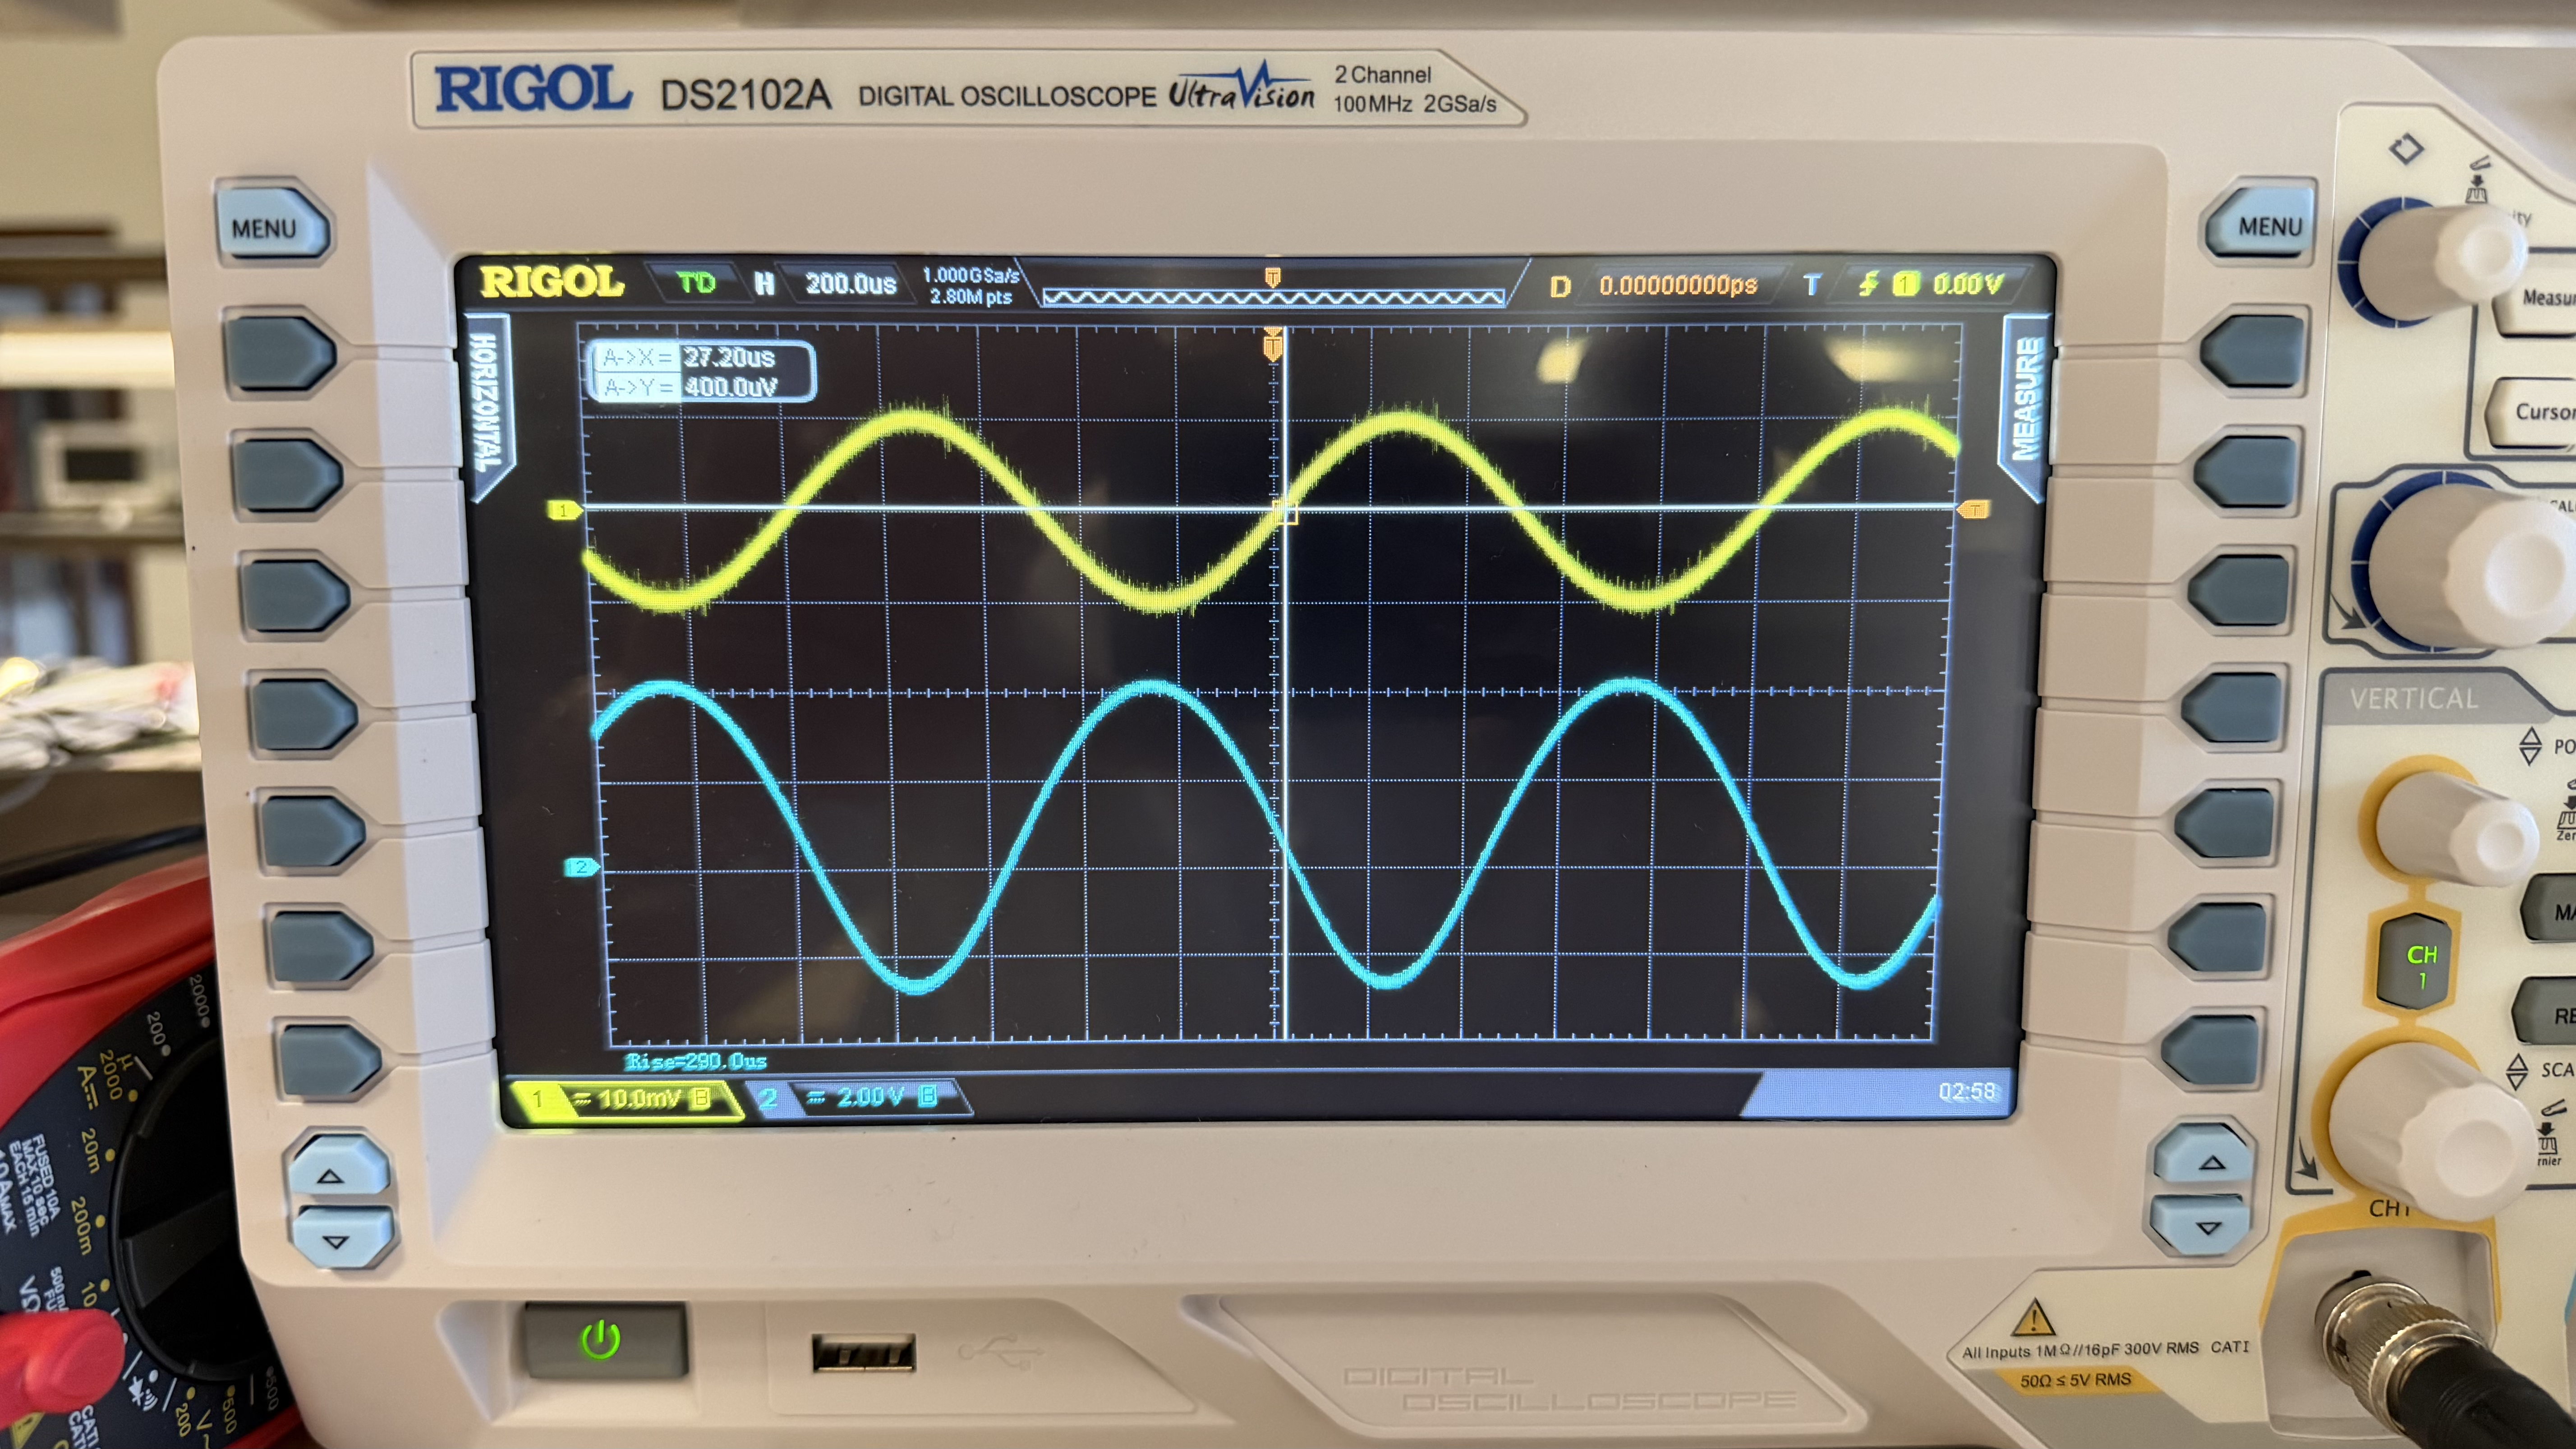
\includegraphics[width=\textwidth]{IMG_0892.png}
    \caption{Open Load ($R_L \approx \SI{1}{M\Omega}$): $v_{open} = \SI{9.60}{V_{pp}}$.}
    \label{fig:open_load}
  \end{subfigure}
  \hfill
  \begin{subfigure}{0.48\textwidth}
    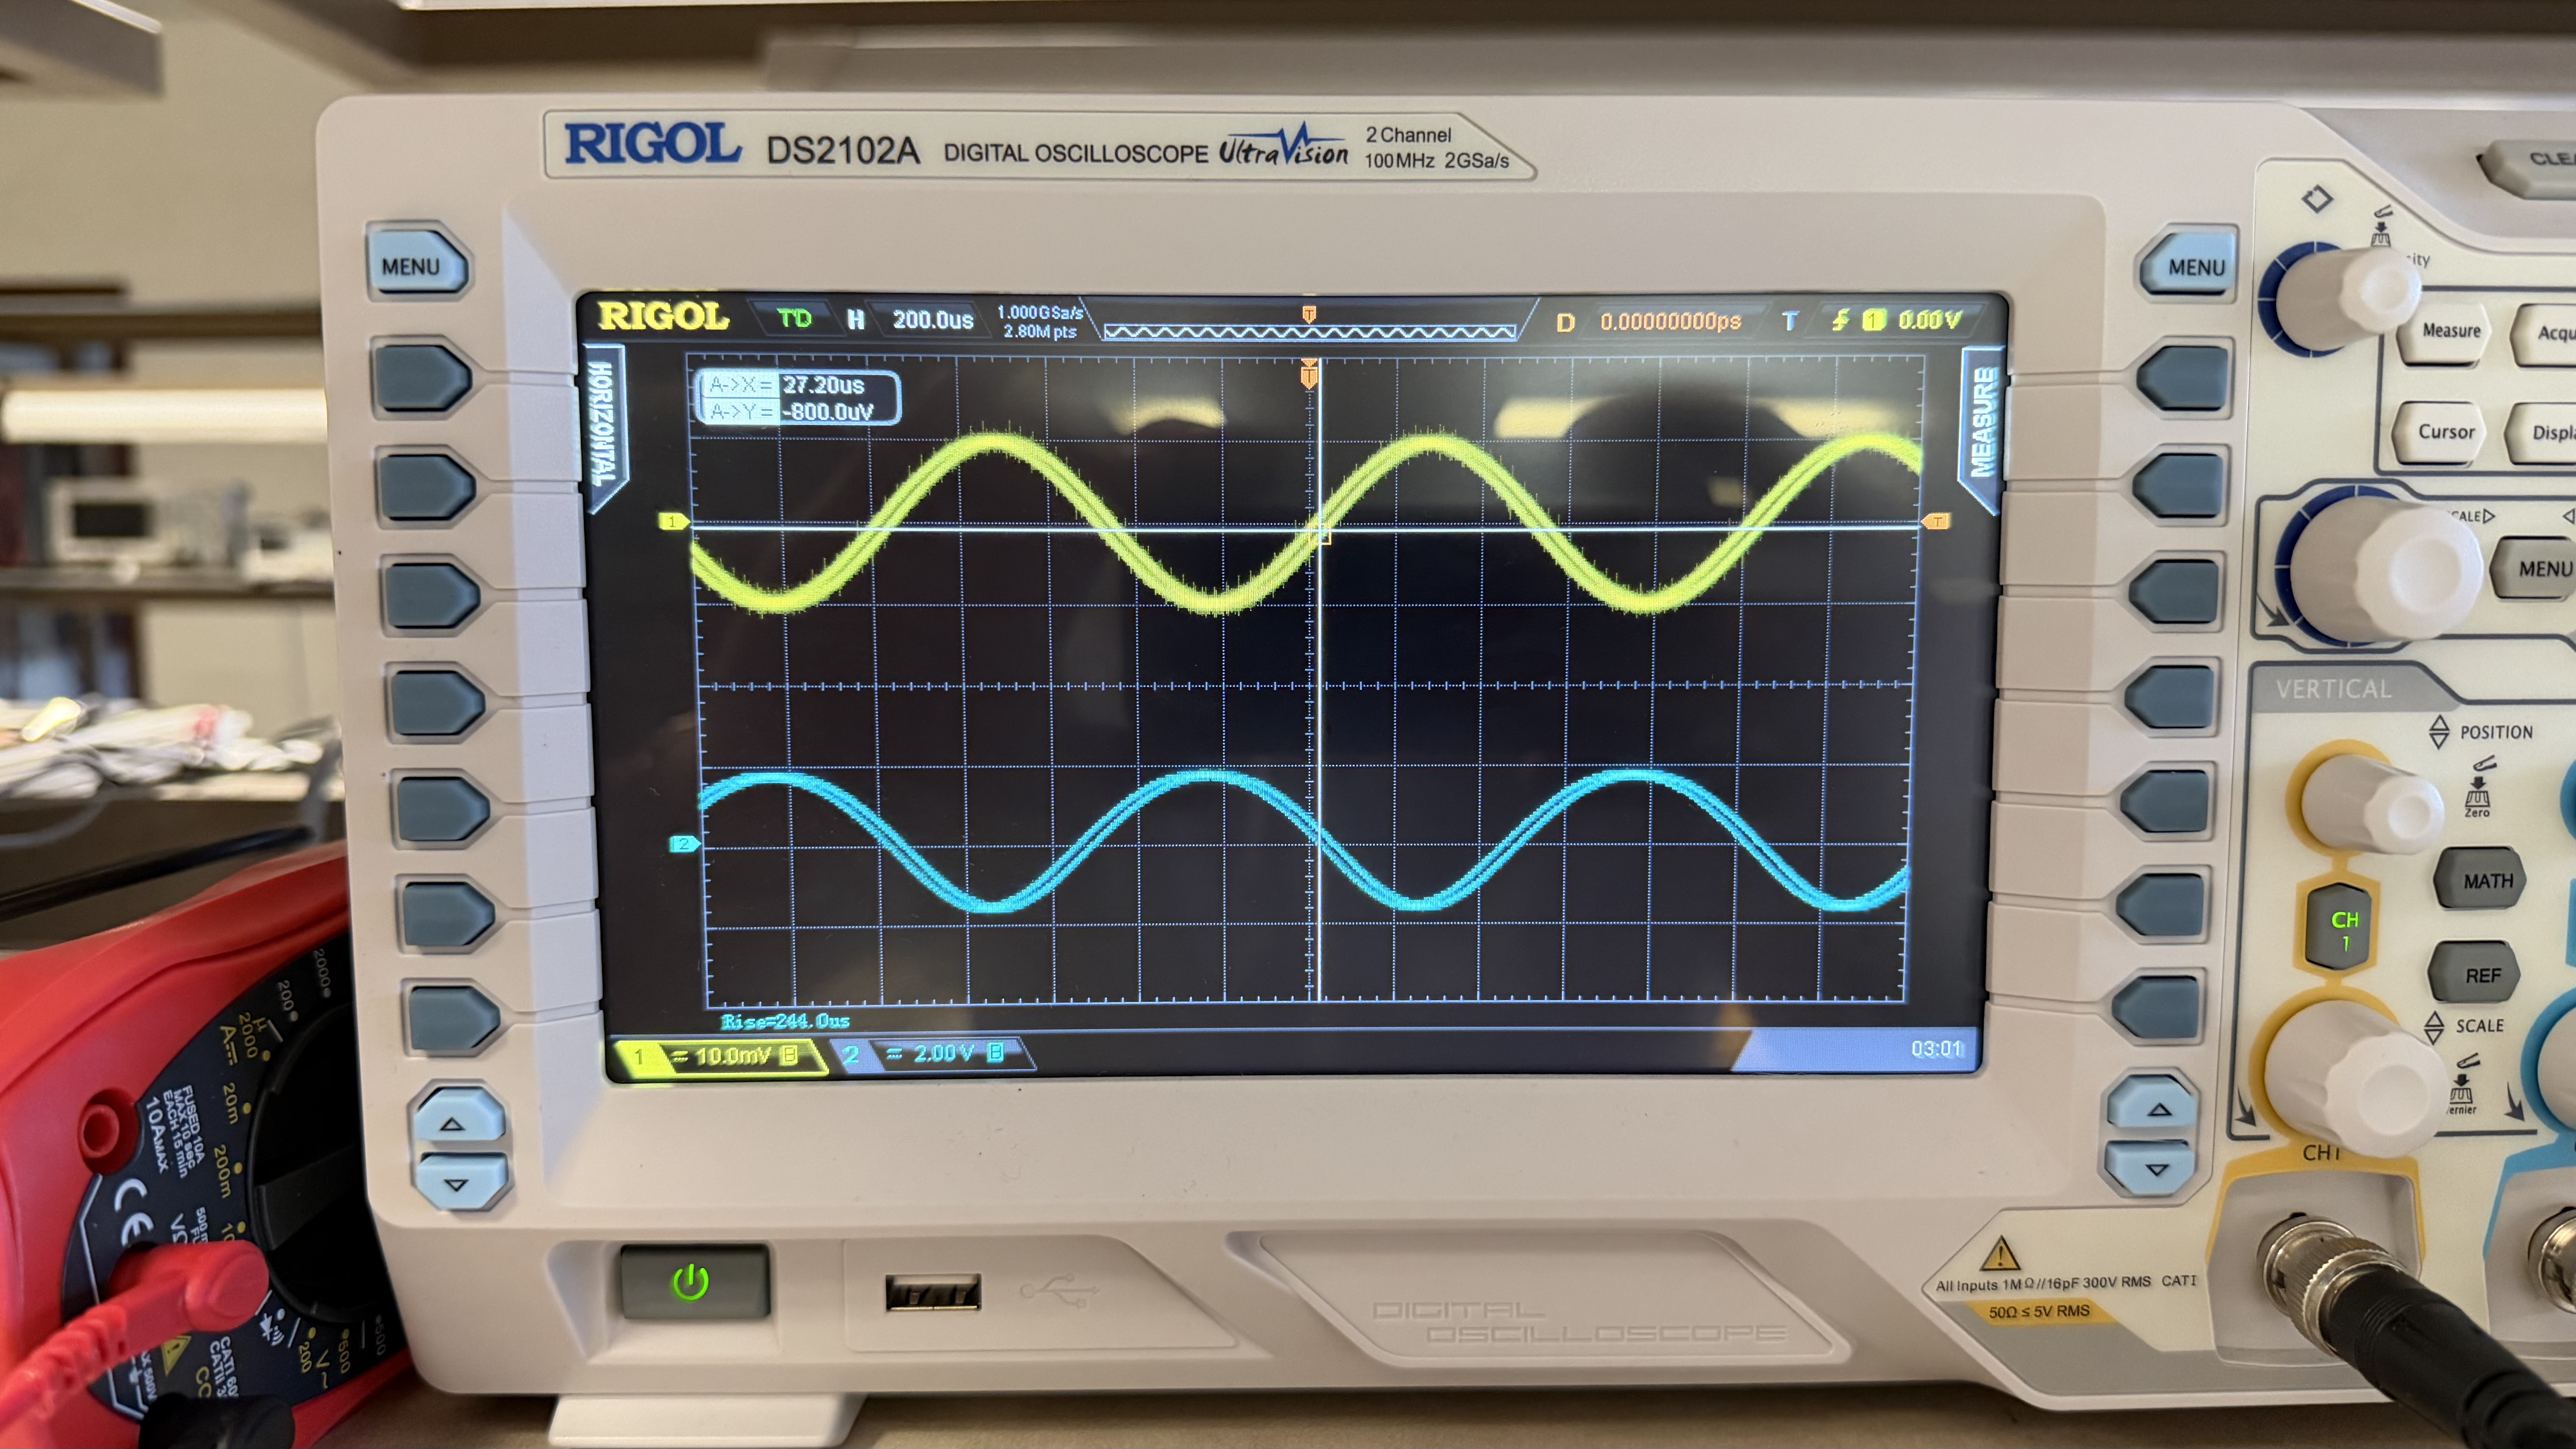
\includegraphics[width=\textwidth]{IMG_0894.png}
    \caption{Loaded ($R_L = \SI{9.1}{k\Omega}$): $v_{loaded} = \SI{4.32}{V_{pp}}$.}
    \label{fig:loaded}
  \end{subfigure}
  \caption{Determination of Output Resistance. Comparing the output voltage between an open load and a $\SI{9.1}{k\Omega}$ load.}
  \label{fig:ro_meas}
\end{figure}

\textbf{Calculation:}
Using the voltage divider relationship:
$$ v_{loaded} = v_{open} \left( \frac{R_L}{R_L + R_o} \right) $$
Solving for $R_o$:
$$ R_o = R_L \left( \frac{v_{open}}{v_{loaded}} - 1 \right) = \SI{9.1}{k\Omega} \left( \frac{9.60}{4.32} - 1 \right) \approx \SI{11.12}{k\Omega} $$

\textbf{Comparison:} This experimental value ($\SI{11.1}{k\Omega}$) is very close to the measured collector resistor value of $R_C = \SI{10.74}{k\Omega}$. This confirms the theory that for a BJT amplifier, $R_o \approx R_C$ (assuming $r_o$ is large).

\subsection{Clipping and Distortion}
To test the dynamic range, the input voltage was increased significantly. Figure \ref{fig:clipping} shows the output waveform distorting (clipping) at the bottom rail.

\begin{figure}[H]
  \centering
  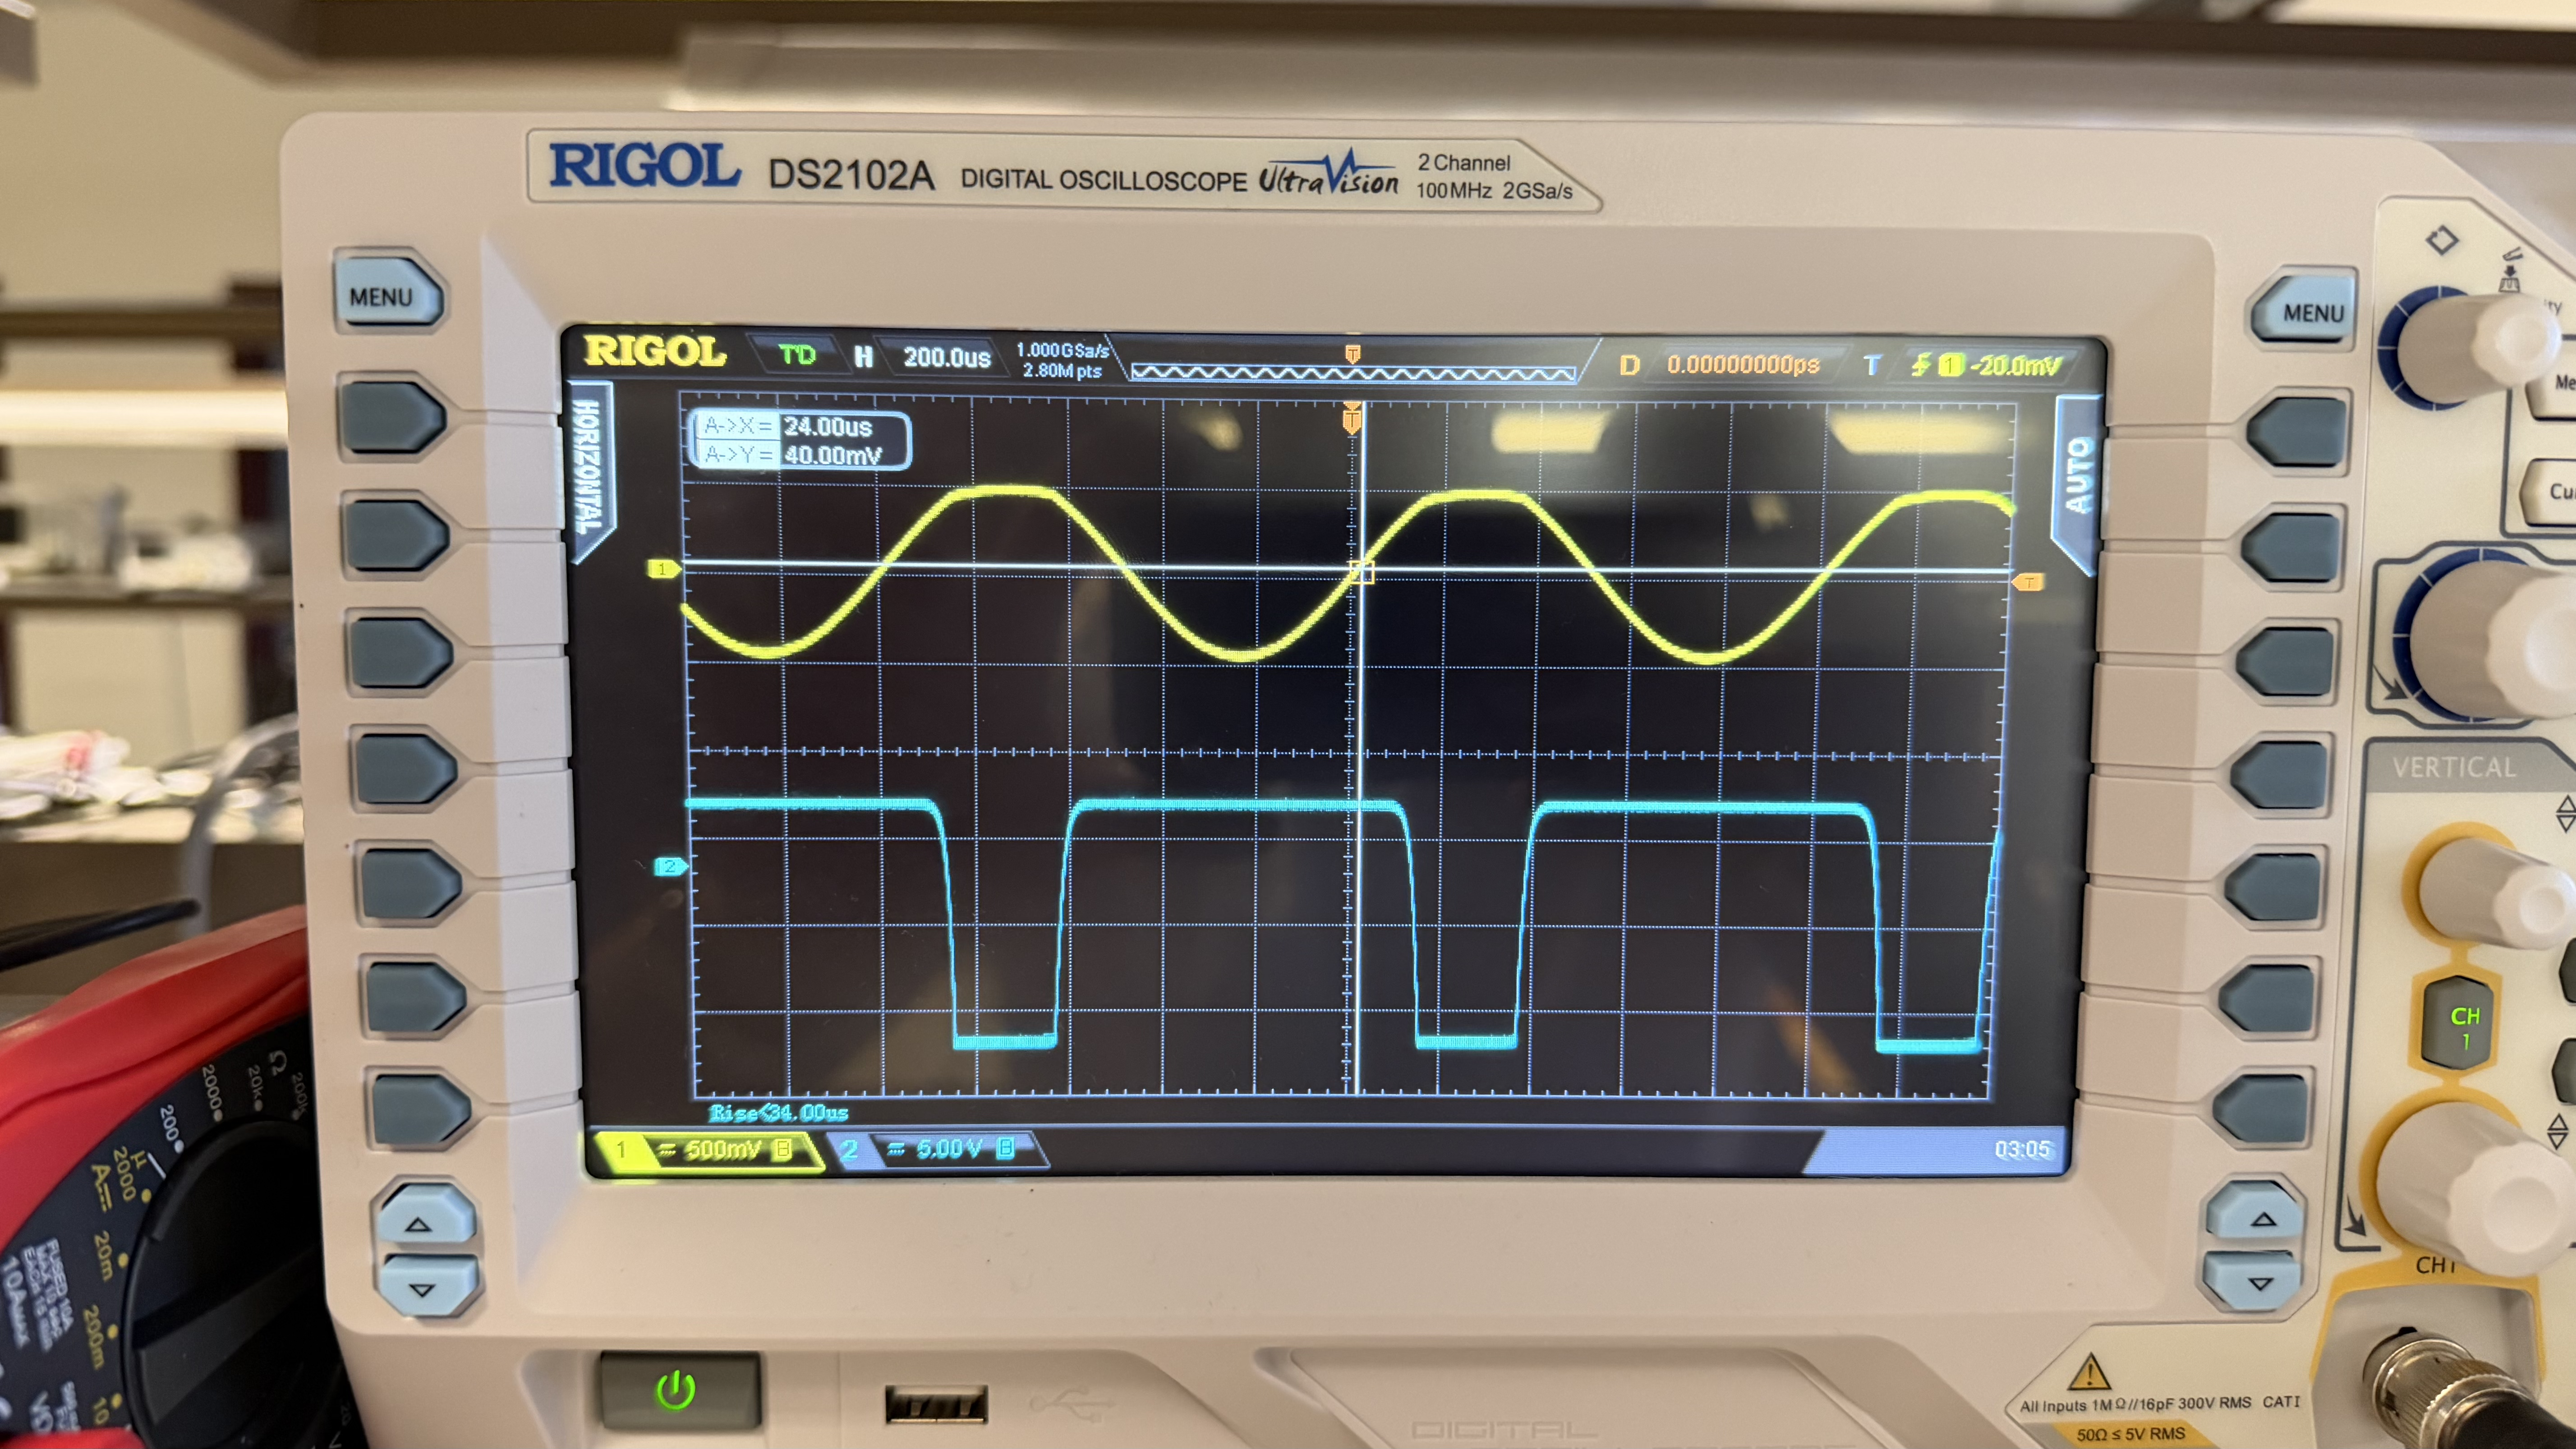
\includegraphics[width=0.7\textwidth]{IMG_0895.png}
  \caption{Output signal showing saturation/clipping when the input amplitude is increased.}
  \label{fig:clipping}
\end{figure}

The clipping occurs because the transistor enters the saturation region when the signal swing exceeds the available headroom defined by the DC operating point and power rails.

\section{Conclusion}
The design of the Common-Emitter amplifier was highly successful.
\begin{enumerate}
  \item The DC bias point was stable with $I_C = \SI{1.01}{mA}$, matching the $\SI{1}{mA}$ target. The measured $V_{BE}$ and $V_{CE}$ values matched theoretical expectations almost perfectly.
  \item The measured AC gain was $\mathbf{-196.8 \text{ V/V}}$, which is within 1.6\% of the $-200 \text{ V/V}$ goal.
  \item The output resistance was measured to be $\SI{11.12}{k\Omega}$, confirming it is dominated by the collector resistor ($R_C$).
\end{enumerate}

% --- BIBLIOGRAPHY ---
\section{Bibliography}
[1] Fixel, Debora. "ENGR 305 - Lab 10: BJT Common-Emitter Amplifier." Trinity College, Hartford, CT, November 2025.
\newline

[2] Jameco Electronics. "2N3904 NPN General Purpose Amplifier." Datasheet, Part no. 38359.

\end{document}
